\documentclass{anstrans}

\title{Coupled Neutronics/Thermal-Hydraulics Simulation of the Molten Salt Fast Reactor with Moltres}
\author{Sun Myung Park and Kathryn D. Huff}
\institute{Dept. of Nuclear, Plasma and Radiological Engineering, University of Illinois at Urbana-Champaign \\
smpark3@illinois.edu}

\usepackage{graphicx} % allows inclusion of graphics
\usepackage{booktabs} % nice rules (thick lines) for tables
\usepackage{microtype} % improves typography for PDF
\usepackage{xspace}
\usepackage{multirow} 
\usepackage{array}
\setlength{\arrayrulewidth}{.4mm}
\renewcommand{\arraystretch}{1.2}
\usepackage[labelfont=bf]{caption}
\captionsetup[table]{name=Table}
\renewcommand{\thetable}{\arabic{table}}
\usepackage{subcaption}
\usepackage{enumitem}
\usepackage{placeins}
\usepackage{siunitx}
\newcolumntype{c}{>{\hsize=.56\hsize}X}
\newcolumntype{b}{>{\hsize=.7\hsize}X}
\newcolumntype{s}{>{\hsize=.74\hsize}X}
\newcolumntype{f}{>{\hsize=.1\hsize}X}
\newcolumntype{a}{>{\hsize=.45\hsize}X}
\usepackage{titlesec}
\titleformat*{\subsection}{\normalfont}

\begin{document}

\begin{abstract}
This summary presents the outline for the code validation of Moltres, a coupled neutronics/thermo-hydraulics simulation tool developed for simulating molten salt reactors, using a modified geometry of the Molten Salt Fast Reactor benchmark model. Homogenised neutron group constant data for each material region were generated using the Monte Carlo neutron transport code Serpent. The data will be fed into Moltres, along with other input parameters such as flow velocity and initial conditions. The steady state and selected accident transient simulation results will be studied and compared against existing results for the MSFR benchmark model. With this study, we will assess the performance of the Moltres code, and identify key technical gaps and areas for improvement.
\end{abstract}

\section{INTRODUCTION}

Moltres is an open source simulation tool developed for simulating molten salt reactors (MSR). It is an application that is developed in Multiphysics Object Oriented Simulation Environment (MOOSE) \cite{gaston_moose:_2009}, a finite-element, multi-physics framework for solving non-linear problems. Through the MOOSE framework, Moltres solves the coupled n-group neutron diffusion, temperature and delayed neutron precursor governing equations on a coarse, adaptive meshing scheme. 

Lindsay et al. \cite{lindsay_introduction_2018} performed a demonstration of Moltres with the Molten Salt Reactor Experiment (MSRE) reactor design developed by Oak Ridge National Laboratory in the 1950s and 60s. The simulation used a 2D-axisymmetric model resembling the MSRE design for proof-of-concept, followed by a 3D geometry also resembling the MSRE design for further analysis. The temperature and neutron flux results from the 3D model were in good agreement with analytical solutions for the MSRE by Briggs et al. \cite{briggs_molten-salt_1964}. Moltres can also be internally coupled with other MOOSE application codes for additional physics to be introduced into MSR simulations.

%In this summary, we will first discuss the motivations for this research. This is followed by a brief description of the advantages of MSRs. Next, we introduce the Molten Salt Fast Reactor (MSFR) design and existing simulation results of the MSFR. The subsequent simulation tools section goes into further detail of the neutronics and thermal-hydraulics implementation in Moltres. The methodology section describes the outline of the code validation exercise of Moltres against other existing MSFR results, after which we discuss and analyse preliminary neutronics results from Serpent in the following section. 

\section{MOTIVATION}

The logical next step in the development of Moltres is its application on other MSR designs. The MSR design of interest for this summary and the subsequent report is the Molten Salt Fast Reactor (MSFR) \cite{serp_molten_2014}. The pool-type MSFR is a fast reactor with a single large pool of fuel-containing molten salt flowing upwards through the center of the core. The fuel salt flow separates at the top into 16 smaller peripheral coolant loops for heat exchange, pumping and other processes before flowing back into the center. As a fast reactor, it has no need for moderators such as the numerous graphite channels in the channel-type epithermal MSRE design.

A number of technical gaps in the Moltres code have to be filled to accurately simulate the physics present in the MSFR, especially during transient and accident scenarios. Some features that will be developed include improvements in the fluid dynamics, as Moltres can currently only handle laminar flow at predetermined velocity distributions. Radiative heat transfer is currently not accounted for, with only heat transfer through conduction and convective flow. Furthermore, there is currently no equivalent implementation of pumps in Moltres; flow velocities are user-defined. This greatly limits the study of transient scenarios involving variations in pump speed. 

By comparing the simulation results with existing literature on the MSFR, we can quantify and assess the impact of these technical gaps, and develop an effective plan for future work on improving Moltres.

%\section{MOLTEN SALT REACTORS}

%A major feature to be introduced is pump and buoyancy driven flow. The current implementation of Moltres requires user-determined velocity values as opposed to having the flow determined by fluid dynamics in the presence of pumps and buoyancy effects due to the expansion of heated molten salt. While this implementation is sufficient for 

%The development of accurate simulation tools for MSRs is an essential step towards their potential deployment. MSRs are arguably much safer than conventional nuclear reactors due to several passive safety mechanisms that make severe accidents extremely unlikely to occur. When core temperatures rise due to unprotected reactivity insertions, the strong negative temperature reactivity coefficients of the fuel salt limit further increases in reactivity and temperature \cite{elsheikh_safety_2013}. The coolant salts are chemically inert and do not react explosively with air or water. Fission products can be continuously removed through online chemical reprocessing and helium sparging. This reduces the radiological impact of a severe accident involving a hull breach and the release of molten salt to the environment \cite{elsheikh_safety_2013}.

%Certain MSR designs also operate with epithermal or fast neutron spectra which can burn off the transuranic elements inevitably produced when using $^{235}$U fuel. Some designs such as the Molten Salt Fast Reactor (MSFR) are designed to breed fissile $^{233}$U from $^{232}$Th \cite{serp_molten_2014}, thereby gaining the advantages of running a thorium fuel cycle. MSRs also typically operate at low pressures compared to light water reactors (LWR) as the operating temperatures are far below the boiling temperatures of the molten salt mixture. This eliminates the need for thick pressure vessels borne from safety constraints \cite{elsheikh_safety_2013}.

\section{THE MOLTEN SALT FAST REACTOR}

The MSFR is a reference design for a fast-spectrum molten salt reactor first developed under the Evaluation and Viability of Liquid Fuel Fast Reactor System (EVOL) project, and continued by the Safety Assessment of the Molten Salt Fast Reactor (SAMOFAR) project \cite{serp_molten_2014}. Figure \ref{fig:msfr} shows a schematic view of the MSFR. The main specifications of the MSFR are given in Table \ref{table:msfr}.

\begin{figure}[t] 
	\centering
	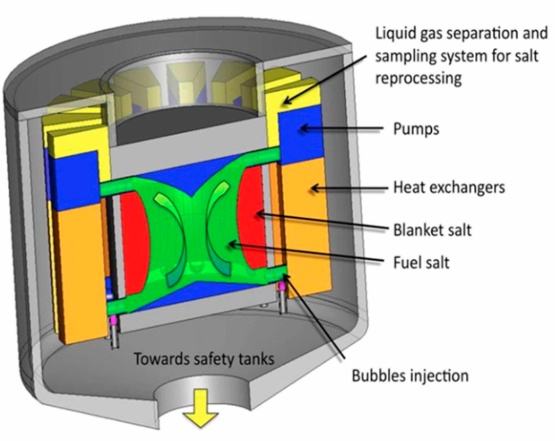
\includegraphics[width=0.48\textwidth]{./figures/MSFR}
	\caption{MSFR reactor design concept \cite{serp_molten_2014}.}
	\label{fig:msfr}
\end{figure} 

\begin{table}
\begin{tabular}{ l l }
\hline
Parameter & Value \\
\hline
Electric/Thermal power [MW$_{\text{e}}$/MW$_{\text{th}}$] & 1300 / 3000  \\
Salt volume [m$^3$] & 18 \\
Salt fraction in core & 0.5 \\
Number of circulation loops & 16 \\
Nominal flow rate [kg s$^{-1}$] & 18500  \\
Nominal circulation time [s] & 4.0 \\
Inlet/outlet temperature [K] & 973 / 1073 \\
Blanket volume [m$^3$] & 7.3\\
\hline
\end{tabular}
\caption{Specifications of the MSFR design \cite{serp_molten_2014}.}
\label{table:msfr}
\end{table}

Lithium fluoride (LiF) is the major component of the fuel and blanket molten salts used for the MSFR. Fissile and fertile isotopes are introduced into the mixture by mole fractions of 77.5\%LiF-22.5\%AcF$_4$, where AcF$_4$ represents actinide fluorides such as uranium and thorium fluorides. The MSFR supports various fuel compositions. It can run on the same $^{235}$U-$^{238}$U fuel used in most conventional LWRs. It can also be run on a mixture of fresh and used uranium fuel containing reprocessed transuranic isotopes \cite{fiorina_investigation_2013}. However, the main configuration of the MSFR is a breeder reactor running on $^{233}$U-$^{232}$Th \cite{merle-lucotte_launching_2011}. Breeding ratios of up to 1.1 have been reported by previous studies on the MSFR \cite{fiorina_molten_2013}. 

The primary fuel salt flows upwards through the 9 m$^3$ central core region. At the top of the core, the flow separates into 16 smaller external loops, each of which passes through a heat exchanger and is pumped back into the core. The primary heat exchangers transfer heat from the fuel salt to an intermediate salt coolant loop. There are other instrumentation along the external loops for online reprocessing and gas sparging. The core is radially surrounded by a tank of blanket molten salt, with reflectors at the top and bottom of the core. The blanket salt contains fertile isotopes such as $^{232}$Th for fuel breeding. There is a layer of neutron absorbing material behind the blanket tanks to protect the heat exchangers, pumps and other instrumentation from neutron irradiation damage.

Various authors have performed a number of steady state and transient multiphysics simulations for the MSFR. A paper by Fiorina et al. \cite{fiorina_modelling_2014} compares results between coupled models developed on the multiphysics code COMSOL and an in-house code developed at Delft University of Technology. The models used 2D axisymmetric models of the MSFR and solved multi-group neutron diffusion equations for the neutronics, and they showed good agreement for some of the transient cases studied. A more comprehensive 3D model has been developed and studied by Aufiero et al. \cite{aufiero_development_2014} using the computional fluid dynamics (CFD) toolbox OpenFOAM. Although this model relied on the one-group neutron diffusion equation, it enabled the study of the full 3D core geometry and 3D transient scenarios such as the failure of one of the 16 pumps in the MSFR.

More recently, a coupled tool, comprising of the thermal-hydraulics code TRACE and a multi-group 3D spatial neutronics solver PARCS, was used to run steady state and transient simulations of the MSFR \cite{pettersen_coupled_2016}. This approach allowed for a 3D model simulation of the MSFR on a coarse mesh, thus improving on the 2D axisymmetric COMSOL/TUDelft models with the benefit of much lower computation times in comparison to the CFD-OpenFOAM models. On top of steady state simulations, the transient scenarios studied by Pettersen \cite{pettersen_coupled_2016} include loss of heat sink, pump over-speed, over-cooling and loss of flow. 

\section{SIMULATION TOOLS}

Moltres is an application code developed in the MOOSE framework \cite{gaston_moose:_2009}. The MOOSE framework solves non-linear equations through the discretization of partial differential equations (PDE) on an adaptive coarse meshing scheme provided by LibMesh \cite{kirk_libmesh:_2006} and PetSc \cite{satish_balay_petsc_2015}. Individual terms of PDEs that define the physics involved in a system are represented in MOOSE (and its applications) by kernels. For example, the various terms in the neutron diffusion equation such as the diffusion term, time evolution term, etc. all have a corresponding physics kernel defined in Moltres. Boundary conditions are also handled in a similar fashion. Moltres can solve for an arbitrary number of neutronics groups as long as the relevant group constants are provided in a Moltres-compatible format.

As mentioned in the previous Moltres study \cite{lindsay_introduction_2018}, the neutronics in Moltres is described by the time-independent multi-group neutron diffusion equation as shown in Equation \ref{eq1}.
\begin{align}
\frac{1}{v_g} &\frac{\partial \phi_g}{\partial t} - \nabla \cdot D_g \nabla \phi_g + \Sigma^r_g \phi_g \nonumber \\ 
&= \sum^G_{g \neq g'} \Sigma^s_{g' \rightarrow g} \phi_{g'} + \chi^p_g \sum^G_{g'=1} (1-\beta) \nu \Sigma^f_{g'} \phi_{g'} + \chi^d_g \sum^I_i \lambda_i C_i \label{eq1}
\end{align}

The delayed neutron precursors are governed by the following equation:
\begin{align}
\frac{\partial C_i}{\partial t} = \sum^G_{g'=1} \beta_i \nu \Sigma^f_{g'} \phi_{g'} - \lambda_i C_i - \frac{\partial}{\partial z} u C_i \label{eq2}
\end{align}

Lastly, the governing equation for temperature in the molten salt is given as:
\begin{align}
\rho_f c_{p,f} \frac{\partial T_f}{\partial t} + \nabla \cdot \big( \rho_f c_{p,f} \overrightarrow{u} \cdot T_f - k_f \nabla T_f \big) = Q_f \label{eq3}
\end{align}
where the source term $Q_f$ is given as:
\begin{align}
Q_f = \sum^G_{g=1} \epsilon_{f,g} \Sigma_{f,g} \phi_g \label{eq4}
\end{align}

The governing equation for temperature in the structural components is similar to that for the molten salt, with exclusion of the advection term.
\begin{align}
\rho_s c_{p,s} \frac{\partial T_s}{\partial t} + \nabla \cdot \big(- k_s \nabla T_s \big) = Q_s \label{eq5}
\end{align}

The mathematical form of $Q_s$, which is the source term in the structural components due to gamma and neutron irradiation upon these components, is yet to be determined.

The group constants are to be generated on Serpent \cite{leppanen_serpent_2015}. Serpent is a versatile continuous-energy Monte Carlo code used in numerous reactor physics applications such as neutron group cross section generation and burnup calculations.

\section{METHODOLOGY}

This study uses a truncated version of an established benchmark MSFR reactor core geometry \cite{pettersen_coupled_2016}. It is a 2D axisymmetric model as shown in Figure \ref{fig:benchmark}. This geometry focuses on the active central region of the core. Basing the geometry on the benchmark model facilitates comparisons with previous MSFR studies by various authors \cite{fiorina_modelling_2014} \cite{pettersen_coupled_2016} on the benchmark model for code validation purposes. More complete geometries may be considered for future work. For Serpent neutronics simulations, the 2D model was extended into a 3D geometry by rotating it around the central axis to form concentric cylinders, as was done by Pettersen \cite{pettersen_coupled_2016}.

We obtained six-group neutronics data from Serpent. The input parameters consisted of the extended 3D geometry, material compositions and densities of the various components in the model, the neutron energy bounds, the JEFF-3.1.2 cross section library, and the temperatures at which the group constants are to be generated.

The fuel salt composition is given in table \ref{table:fuelsalt}. The fissile $^{233}$U composition is 1\% higher than that used by Pettersen \cite{pettersen_coupled_2016} to reach criticality at 1030 K with our modified geometry. The temperature-dependent density formulae used are all unchanged from the aforementioned paper. The simulated temperatures range from 900 K to 1200 K at 50 K intervals. This range covers the expected operating temperature range of the MSFR. The neutron energy group upper bounds are given in table \ref{table:bound}. These group boundaries were chosen to match the boundaries used by Pettersen \cite{pettersen_coupled_2016} and Fiorina \cite{fiorina_modelling_2014}.

The Serpent output data relevant to Moltres are the fission cross section, fission neutron production cross section, removal cross section, average energy deposited per fission, inverse neutron speed, average neutron yield, neutron flux, total fission spectrum, delayed fission spectrum, diffusion coefficient and scattering production matrix for each of the six neutron energy groups. Serpent also provides eight-group delayed neutron fractions and decay constants for use in Moltres. Preliminary Serpent results were obtained and are discussed in the next section.

The input parameters required by Moltres include flow velocity, the number of neutron and delayed neutron precursor groups, multi-group neutronics data, the geometry mesh file, appropriate initial temperature values, neutronics and temperature boundary conditions, and material properties. Material properties include thermal conductivity, specific heat capacity and density. Moltres automatically interpolates the temperature-dependent group constant data that it is provided, to obtain group constant data values for all temperatures between 900 K and 1200 K. 

The coupled neutronics and thermal-hydraulics simulation starts from the initial temperatures and is expected to converge to steady state temperature and neutron flux distributions over time for the given fuel salt composition. From this steady state, transient accident scenarios that can be studied through varying the flow velocity and fuel salt composition.
%
\begin{table}[t]
\centering
\begin{tabular}{rr}
\hline
{Isotope} & {Mole fraction [\%]}\\
\hline
$^7$Li & 29.0\\
$^{19}$F & 62.6\\
$^{232}$Th & 7.39\\
$^{233}$U & 1.01\\
\hline
\end{tabular}
\captionsetup{justification=centering}
\caption{Fuel salt composition used for the Serpent simulation.}
\label{table:fuelsalt}
\end{table}
%
\begin{table}[t]
\centering
\begin{tabular}{ll}
\hline
{Group number} & {Upper bound [MeV]}\\
\hline
1 & 7.485$\times 10^{-4}$\\
2 & 5.5308$\times 10^{-3}$\\
3 & 2.47875$\times 10^{-2}$\\
4 & 0.4979\\
5 & 2.2313\\
6 & 20\\
\hline
\end{tabular}
\captionsetup{justification=centering}
\caption{Neutron energy group upper bounds used in Serpent.}
\label{table:bound}
\end{table}
%
\begin{figure}[h!] 
	\centering
	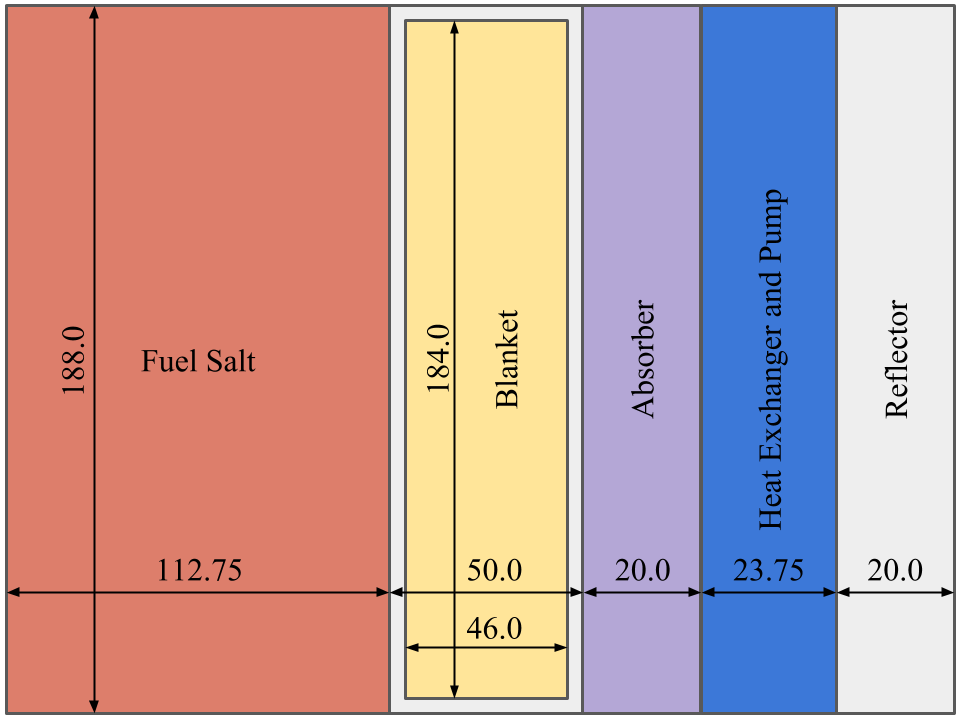
\includegraphics[width=0.46\textwidth]{./figures/benchmark}
	\captionsetup{justification=centering}
	\caption{Cross-section of the 2D axisymmetric model used for the simulation. Derived from the 2D axisymmetric benchmark model of the MSFR \cite{pettersen_coupled_2016}. The figure is not to scale.}
	\label{fig:benchmark}
\end{figure} 
%
\section{PRELIMINARY NEUTRONICS RESULTS}

The effective multiplication factor $k_{eff}$ and temperature reactivity coefficient $\alpha_T$ values obtained from Serpent are compared with the Serpent results from Pettersen. The model used in that paper is the full 2D axisymmetric benchmark model that includes the fuel inlet and outlet, and reflectors above and below the geometry considered in our Serpent simulations.

The $k_{eff}$ values obtained are shown in table \ref{table:keff}; all values have equal uncertainty values of $\pm 5$ pcm. The $k_{eff}$ at 1030 K is larger than the value reported by Pettersen by 91 pcm as shown in table \ref{table:keffcomp}. This discrepancy grows to 126 pcm at 1200 K. This may be largely due to the 0.01\% increase in mole fraction of fissile $^{233}$U and corresponding decrease in $^{232}$Th used to keep the model critical at 1030 K as compared to Pettersen's model.
%
\begin{align}
\alpha = \frac{k_2 - k_1}{k_1 \Delta T} \label{eq6}
\end{align}

The $\alpha_T$ in table \ref{table:reactivity} was calculated using equation \ref{eq6} for a fair comparison with Pettersen's result, where $k_1$ and $k_2$ are the $k_{eff}$ values at 900 K and 1200 K respectively, and $\Delta T$ is 300 K. Our $\alpha_T$ values larger in magnitude by 0.12 pcm K$^{-1}$. This may also be due to the larger fissile inventory as mentioned above.

It is worth noting that our model is just subcritical when using the same fuel salt composition as Pettersen. However, the $k_{eff}$ value is very close to 1 and the differences may lie in the exact isotopic compositions defined in the input parameters for Serpent. For example, Pettersen used the JEFF-3.1.1 cross section library while we utilised the JEFF-3.1.2 cross section library. Furthermore, the geometry of our models are different; our model truncates the top and bottom fuel salt inlet and outlet regions, and the reflector regions beyond those regions. This choice was made as Moltres will be using this geometry for the coupled neutronics and thermal-hydraulics studies.

The discrepancies in $k_{eff}$ and $\alpha_T$ are deemed to be small, especially as the $\alpha_T$ values are within ~2\% of each other. This shows that the model we have chosen is reasonably close to the MSFR benchmark model.

\section{Conclusion}

We have outlined the methodology for the code validation of Moltres with existing results for the MSFR benchmark model. The preliminary Serpent neutronics results show that the model to be used for this code validation agrees very closely to the existing results by the comparison of the $k_{eff}$ and $\alpha_T$ values within the relevant temperature ranges. Therefore, the proposed model is acceptable for use in the code validation of Moltres.

With this study, key techological gaps and areas for improvement in Moltres will be identified. These will guide future work for the implementation and correction of important physics in molten salt reactors in the Moltres code.
%
\begin{figure}[h!] 
	\centering
	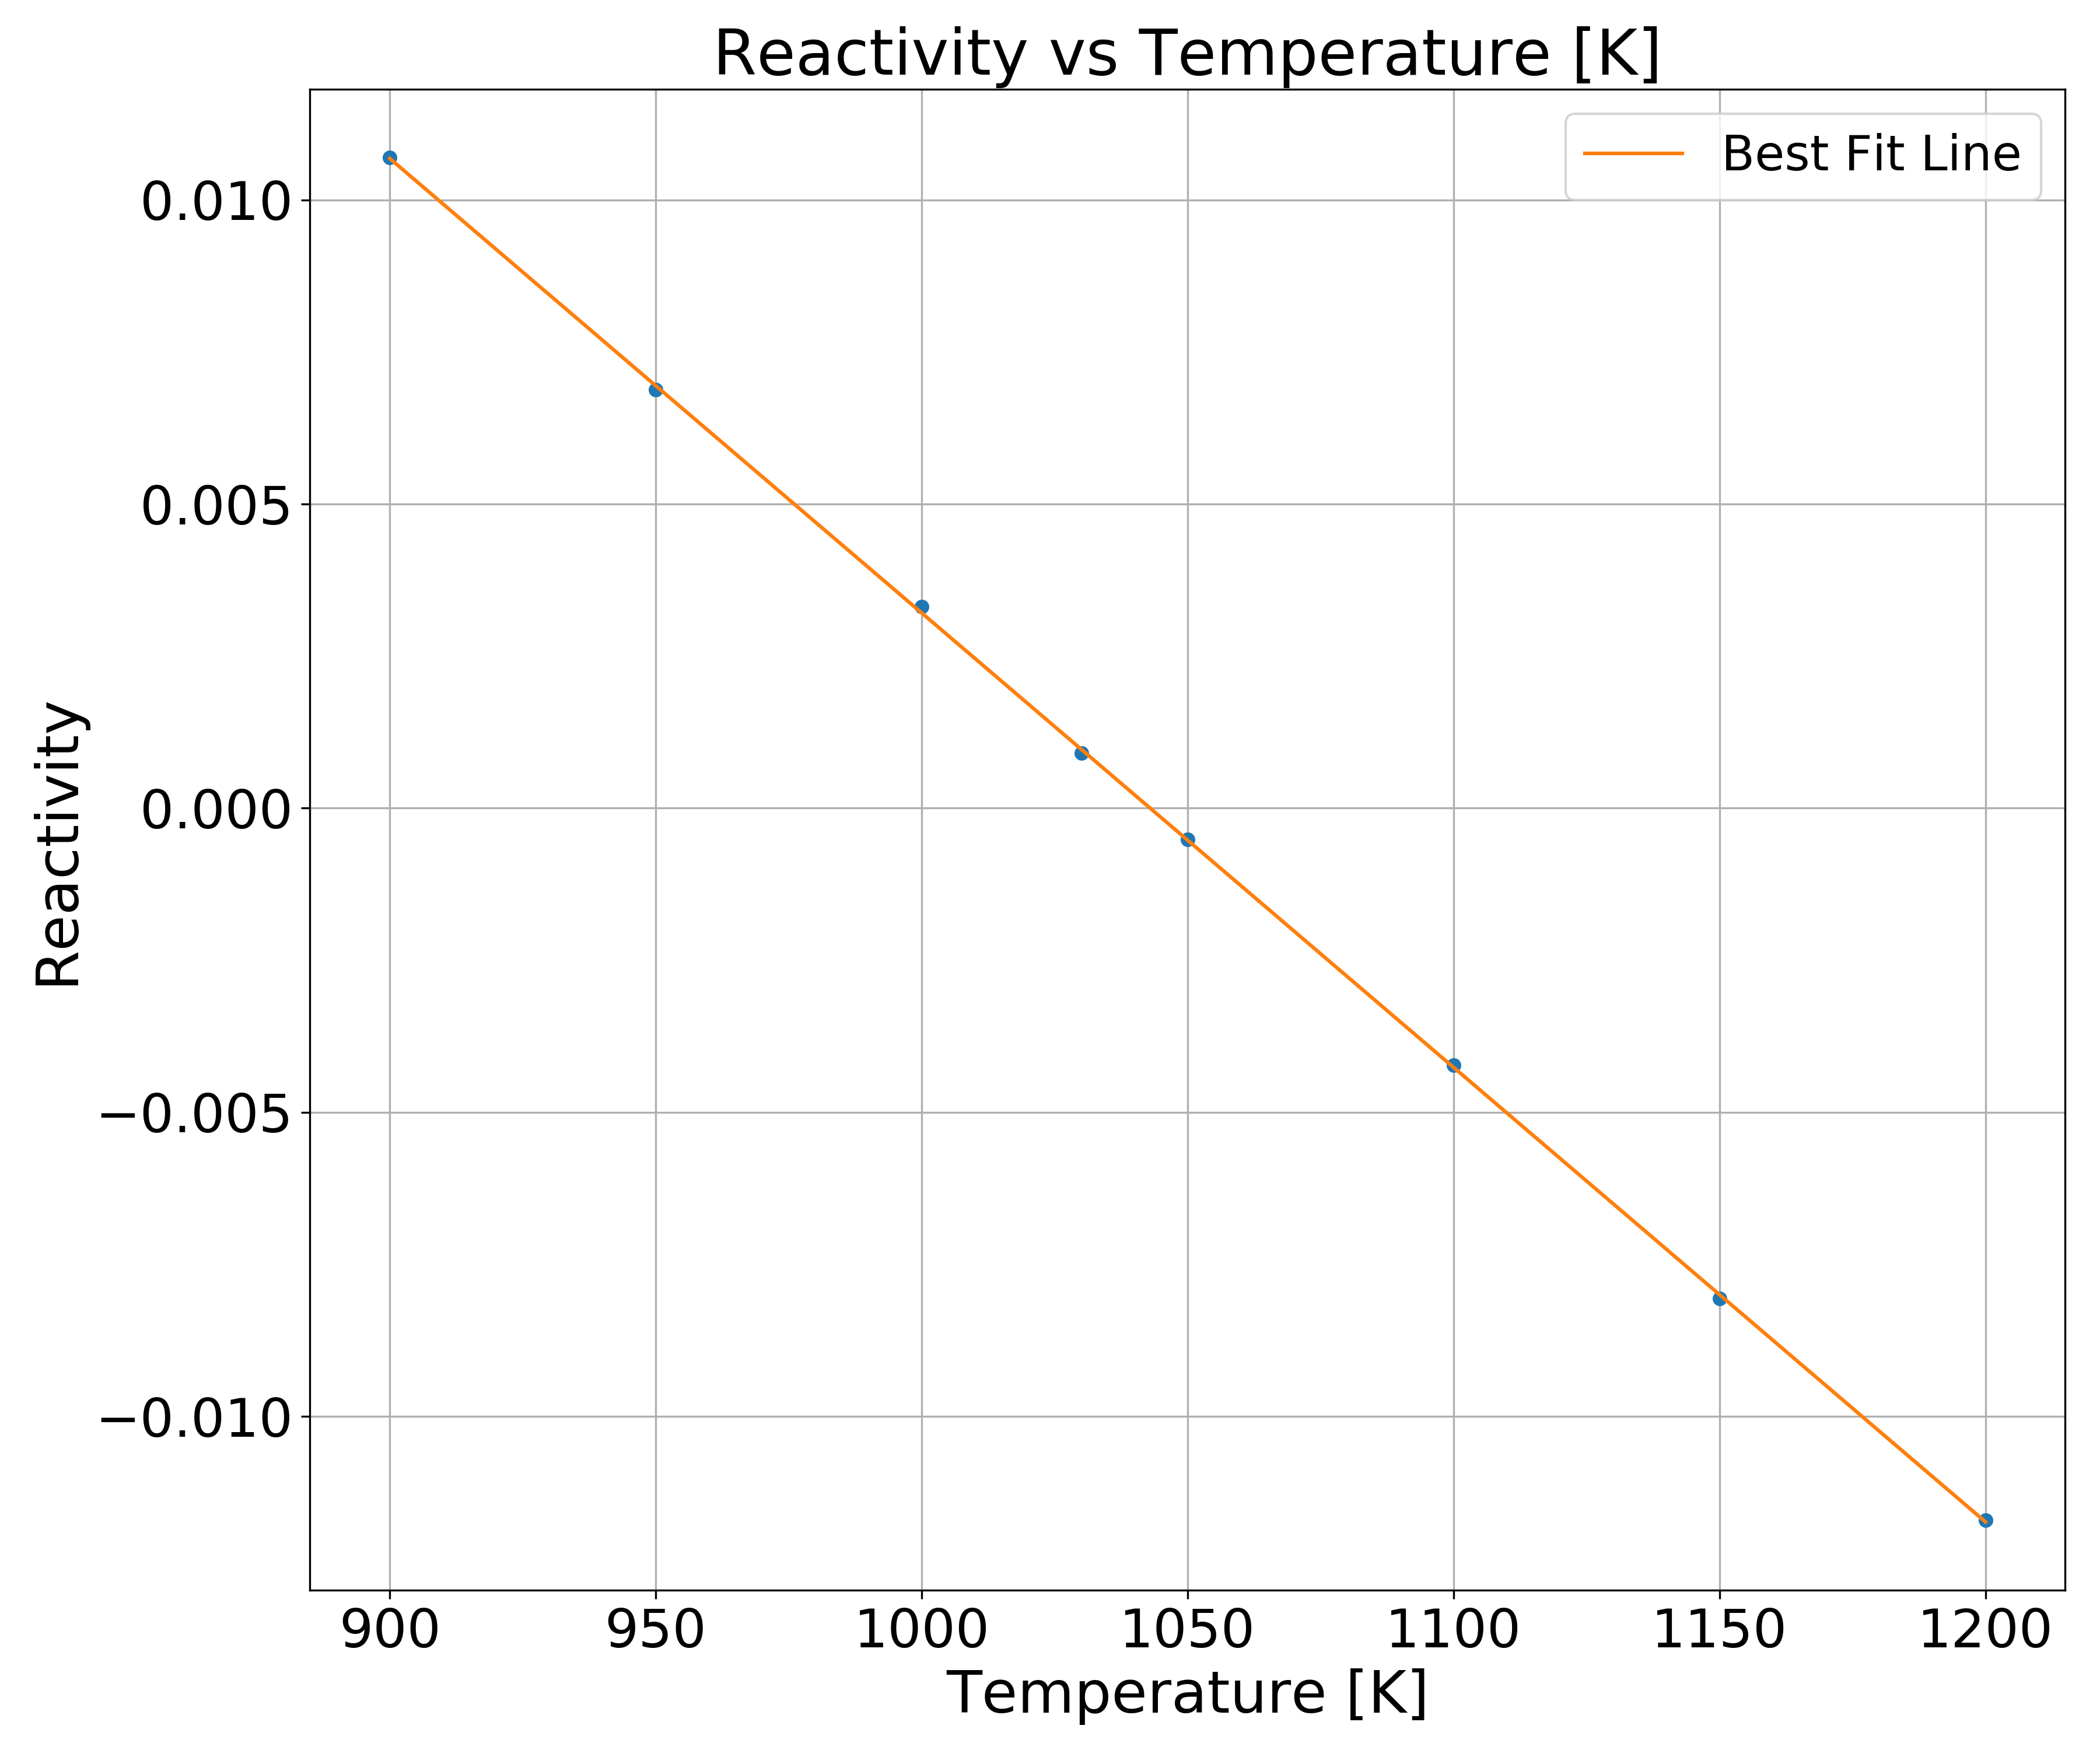
\includegraphics[width=0.48\textwidth]{./figures/reactivityplot}
	\captionsetup{justification=centering}
	\caption{Plot of reactivity vs temperature from Serpent.}
	\label{fig:reactivity}
\end{figure} 
%
\begin{table}[h!]
\centering
\begin{tabular}{ll}
\hline
{Temperature [K]} & {$k_{eff}$}\\
\hline
900 & 1.01081\\
950 & 1.00693\\
1000 & 1.00332\\
1030 & 1.00091\\
1050 & 0.999482\\
1100 & 0.995789\\
1150 & 0.992008\\
1200 & 0.988428\\
\hline
\end{tabular}
\captionsetup{justification=centering}
\caption{Neutron energy group upper bounds used in Serpent.}
\label{table:keff}
\end{table}
%
\begin{table}[h!]
\centering
\begin{tabular}{lll}
\hline
{Source} & {$k_{eff}$ at 1030 K} & $k_{eff}$ at 1200 K\\
\hline
Self (Serpent) & 1.00091 & 0.988428\\
Pettersen (Serpent) & 1.00000 & 0.98716\\
\hline
\end{tabular}
\captionsetup{justification=centering}
\caption{Comparison of $k_{eff}$ values from our Serpent results and Pettersen's results.}
\label{table:keffcomp}
\end{table}
%
\begin{table}[h!]
\centering
\begin{tabular}{ll}
\hline
{Source} & {$\alpha_T$ [pcm K$^{-1}$]}\\
\hline
Self (Serpent) & $-7.39 \pm 0.03$\\
Pettersen (Serpent) & $-7.27 \pm 0.02$\\
\hline
\end{tabular}
\captionsetup{justification=centering}
\caption{Neutron energy group upper bounds used in Serpent.}
\label{table:reactivity}
\end{table}
%

\bibliographystyle{ans}
\bibliography{bibliography}

\end{document}
